\documentclass[10pt,a4paper]{article}
\usepackage[T1]{fontenc}
\usepackage[utf8]{inputenc}
\usepackage{lmodern}
\usepackage{microtype}
\usepackage[margin=0.80in]{geometry}
\usepackage{graphicx}
\usepackage{booktabs}
\usepackage{array}
\usepackage{tabularx}
\usepackage{xcolor}
\usepackage{amsmath,amssymb}
\usepackage[hidelinks]{hyperref}
\usepackage{titlesec}
\usepackage{caption}
\usepackage{float}
\usepackage{enumitem}
\usepackage{tikz}
\usetikzlibrary{positioning,arrows.meta}

\definecolor{ink}{HTML}{111111}
\definecolor{ink2}{HTML}{555555}
\definecolor{soft}{HTML}{ECECEC}
\definecolor{mid}{HTML}{BEBEBE}

\titleformat{\section}{\normalfont\large\bfseries\color{ink}}{\thesection}{0.55em}{}
\titlespacing*{\section}{0pt}{1.0em}{0.35em}
\titleformat{\subsection}{\normalfont\normalsize\bfseries\color{ink}}{\thesubsection}{0.5em}{}
\titlespacing*{\subsection}{0pt}{0.72em}{0.28em}
\titleformat{\paragraph}[runin]{\normalfont\normalsize\bfseries\color{ink}}{}{0pt}{}[:]
\titlespacing*{\paragraph}{0pt}{0.5em}{0.45em}
\captionsetup{font=small,labelfont=normalfont,textfont=normalfont,skip=4pt}
\setlist[itemize]{leftmargin=1.3em,itemsep=2pt,topsep=3pt,parsep=0pt}
\setlist[enumerate]{leftmargin=1.55em,itemsep=2pt,topsep=3pt,parsep=0pt}
\setlength{\textfloatsep}{9pt plus 2pt minus 2pt}
\setlength{\intextsep}{9pt plus 2pt minus 2pt}
\setlength{\floatsep}{7pt plus 2pt minus 2pt}
\setlength{\parindent}{1.15em}
\setlength{\parskip}{0pt}
\linespread{1.02}
\pagestyle{plain}
\raggedbottom

\begin{document}

\begin{center}
{\LARGE\bfseries MK-UNet-CC}\\[3pt]
{\large Conditional and Sparse Multi-Kernel Computation}\\
{\normalsize for Lightweight Medical Image Segmentation}\\[6pt]
{\small Research Proposal - Path A: Methodological Enhancement}\\[3pt]
{\normalsize M. Mohaiminul Islam}\\[4pt]
{\footnotesize Extension of MK-UNet~\cite{rahman2025mkunet}. Preliminary experiments were run on CPU-only hardware.}
\end{center}
\vspace{0.25em}
\noindent\rule{\linewidth}{0.45pt}
\vspace{0.3em}

\noindent
This proposal studies one practical limitation of MK-UNet: its multi-kernel block always computes the same three branches for every input. The project tests whether input-dependent routing can keep segmentation quality while reducing unnecessary branch computation, and whether those savings appear in measured inference latency.


\section{Motivation and Significance}

Point-of-care devices, portable endoscopy systems, and handheld imaging systems may have limited or no dedicated GPU resources. This makes small segmentation models important when memory, computation, and latency are limited. MK-UNet was designed for this setting. Its standard model is reported with 0.316 M parameters and 0.314 G FLOPs, while MK-UNet-T has about 0.027 M parameters~\cite{rahman2025mkunet}. The paper also reports competitive segmentation results across six binary medical-image benchmarks. However, MK-UNet always computes all three depth-wise kernel branches $\{1,3,5\}$ and combines them with the fixed sum
\[
F=F_1+F_3+F_5.
\]
The BUSI ablation shows that kernel choice matters: DICE rises from 70.83 with only a $1\times1$ kernel to 78.04 with $\{1,3,5\}$~\cite{rahman2025mkunet}. Still, the same three-branch computation is used for every input and at every stage.

Different images may not need the same receptive fields. A large polyp, a small lesion, and an uncertain boundary can require different amounts of local and wider context. The central motivation of this proposal is therefore simple: if the useful kernel branch depends on the input, computing every branch every time may waste work. This study asks whether MK-UNet can make that choice dynamically and whether branch skipping produces a real latency benefit, not only a lower FLOP count.

\paragraph{Research question and objectives} Can MK-UNet select and execute kernel branches according to the input while keeping segmentation quality and the lightweight design? The study has three main objectives: (1) test input-dependent branch weighting, (2) test sparse top-1 routing that skips unused branches at inference, and (3) use routing statistics to identify branches that can be removed from a smaller static model. Predictive entropy is also tested as a supporting routing signal rather than as the main novelty.

\section{Problem Definition and Gap in Related Work}

The technical problem is that MKDC contains several useful receptive fields but always executes the same three branches. A useful extension must therefore answer two questions together: can the model choose kernel branches from the input, and can that choice reduce real inference cost after router overhead is included?

\paragraph{Recent related work} Recent medical segmentation studies show that dynamic convolution is already an active direction. LightAWNet uses dynamic convolution in a lightweight segmentation network and reports parameter count, GFLOPs, and execution time~\cite{wang2025lightawnet}. AD-LA Former uses auto-dynamic convolution with location attention to adapt features to different inputs~\cite{wang2025adlaformer}. SEDyConv introduces input-dependent multi-dimensional dynamic convolution and dynamic switches for 3D multi-organ CT segmentation~\cite{hao2025sedyconv}. More recently, SGDC uses structure-guided dynamic kernels and gating to preserve fine boundary information~\cite{shi2026sgdc}. These studies support adaptive convolution for medical segmentation, but they do not report the same experiment studied here: explicit top-1 skipping of MK-UNet's parallel depth-wise branches in an ultra-small MK-UNet-T model.

\paragraph{Research gap and positioning} The novelty is therefore not dynamic convolution by itself. The open question is whether conditional multi-kernel execution is still useful when the full segmentation model has only about 0.027 M parameters~\cite{rahman2025mkunet}. At this scale, router cost and branch-dispatch overhead can be large relative to the backbone. This proposal focuses on true branch skipping, routing-guided static pruning, and measured batch-1 latency rather than assuming that lower FLOPs will produce the same reduction in runtime.

\begin{center}\small
\renewcommand{\arraystretch}{1.08}
\begin{tabularx}{\linewidth}{@{}p{2.55cm}p{3.0cm}p{3.0cm}X@{}}
\toprule
Recent work & Main adaptive idea & Efficiency evidence & Sparse branch execution \\
\midrule
LightAWNet~\cite{wang2025lightawnet} & Dynamic convolution & Params, GFLOPs, time & Not reported \\
AD-LA Former~\cite{wang2025adlaformer} & Auto-dynamic convolution & Internal scaling / redundancy reduction & Not reported \\
SEDyConv~\cite{hao2025sedyconv} & Dynamic convolution + switches & Small parameter growth & Not reported \\
SGDC~\cite{shi2026sgdc} & Structure-guided dynamic kernels & Accuracy / boundary focus & Not reported \\
MK-UNet-T~\cite{rahman2025mkunet} & Fixed $\{1,3,5\}$ MKDC & 0.027 M parameters, throughput & No \\
This proposal & Input-conditioned top-1 routing & Executed FLOPs + batch-1 latency & Yes \\
\bottomrule
\end{tabularx}
\end{center}

The preliminary measurements already show why runtime must be measured directly: in one sparse top-1 run, reported FLOPs fell by about 54\%, while measured batch-1 CPU latency fell by about 13.3\%.

\section{Solution Direction, Proposed Method, and Framework}

The proposed solution changes MKDC in controlled stages so that each experiment answers one clear question. The study first tests soft input-dependent weighting, then adds a difficulty signal, then moves to true branch skipping, and finally uses routing statistics to design a smaller static model. Figure~\ref{fig:framework} summarises this progression.

\begin{figure}[H]
\centering
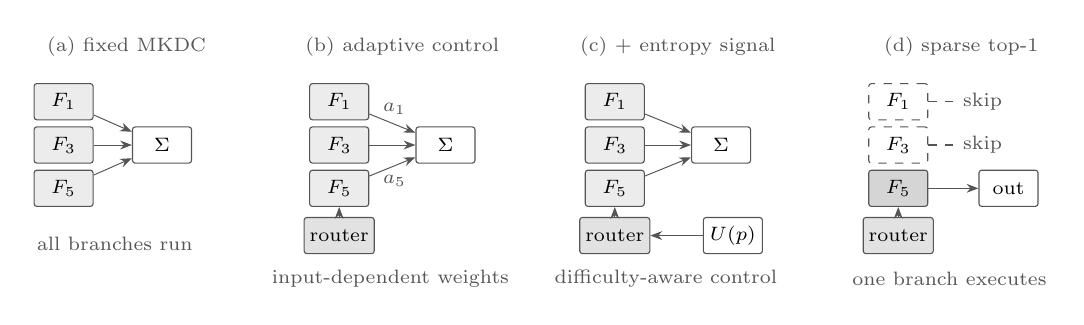
\begin{tikzpicture}[font=\scriptsize,
  box/.style={draw=ink2,rounded corners=1pt,minimum height=4.6mm,minimum width=7.5mm,inner sep=2pt},
  br/.style={box,fill=soft}, rt/.style={box,fill=mid!45},
  lbl/.style={ink2}, ar/.style={-{Stealth[length=1.5mm]},draw=ink2,line width=0.35pt},
  skip/.style={draw=ink2,dashed,line width=0.45pt}]
\node[lbl] at (0,1.5) {(a) fixed MKDC};
\node[br] (a1) at (-0.8,0.8) {$F_1$}; \node[br] (a3) at (-0.8,0.25) {$F_3$};
\node[br] (a5) at (-0.8,-0.3) {$F_5$}; \node[box] (as) at (0.45,0.25) {$\Sigma$};
\foreach \n in {a1,a3,a5} {\draw[ar] (\n) -- (as);}
\node[lbl,align=center] at (-0.15,-1.0) {all branches run};
\begin{scope}[xshift=3.5cm]
\node[lbl] at (0,1.5) {(b) adaptive control};
\node[br] (b1) at (-0.8,0.8) {$F_1$}; \node[br] (b3) at (-0.8,0.25) {$F_3$};
\node[br] (b5) at (-0.8,-0.3) {$F_5$}; \node[rt] (brr) at (-0.8,-0.9) {router};
\node[box] (bs) at (0.55,0.25) {$\Sigma$};
\draw[ar] (b1) -- node[above,pos=.55,lbl]{$a_1$} (bs);
\draw[ar] (b3) -- (bs); \draw[ar] (b5) -- node[below,pos=.55,lbl]{$a_5$} (bs);
\draw[ar] (brr) -- (b5);
\node[lbl,align=center] at (-0.15,-1.45) {input-dependent weights};
\end{scope}
\begin{scope}[xshift=7.0cm]
\node[lbl] at (0,1.5) {(c) + entropy signal};
\node[br] (c1) at (-0.8,0.8) {$F_1$}; \node[br] (c3) at (-0.8,0.25) {$F_3$};
\node[br] (c5) at (-0.8,-0.3) {$F_5$}; \node[rt] (cr) at (-0.8,-0.9) {router};
\node[box,fill=white] (cu) at (0.7,-0.9) {$U(p)$};
\node[box] (cs) at (0.55,0.25) {$\Sigma$};
\foreach \n in {c1,c3,c5} {\draw[ar] (\n) -- (cs);}
\draw[ar] (cr) -- (c5); \draw[ar] (cu) -- (cr);
\node[lbl,align=center] at (-0.15,-1.45) {difficulty-aware control};
\end{scope}
\begin{scope}[xshift=10.6cm]
\node[lbl] at (0,1.5) {(d) sparse top-1};
\node[br,dashed,fill=white] (d1) at (-0.8,0.8) {$F_1$};
\node[br,dashed,fill=white] (d3) at (-0.8,0.25) {$F_3$};
\node[br,fill=mid!65] (d5) at (-0.8,-0.3) {$F_5$};
\node[rt] (dr) at (-0.8,-0.9) {router}; \node[box] (do) at (0.6,-0.3) {out};
\draw[ar] (d5) -- (do);
\draw[skip] (d1) -- ++(0.7,0) node[right,ink2]{skip};
\draw[skip] (d3) -- ++(0.7,0) node[right,ink2]{skip};
\draw[ar] (dr) -- (d5);
\node[lbl,align=center] at (-0.15,-1.45) {one branch executes};
\end{scope}
\end{tikzpicture}
\caption{Proposed study path. The adaptive and entropy-conditioned controls still compute all three branches. Sparse top-1 executes only the selected branch at inference.}
\label{fig:framework}
\end{figure}

\paragraph{A. Feature-adaptive soft routing} A small router uses global average pooling and two $1\times1$ layers to predict three branch weights. The output is
\[
F=\sum_k a_k(x)F_k, \qquad a=K\,\mathrm{softmax}(z/T).
\]
The final router layer starts at zero, so all three weights start at 1.0. This makes the initial output equal to the original MKDC sum; the equality was checked with \texttt{torch.allclose}. This arm tests adaptive weighting but does not save branch computation.

\paragraph{B. Difficulty conditioning} The decoder produces coarse predictions that are not used by the original binary loss. Their normalised predictive entropy is
\[
U(p)=-\frac{p\log p+(1-p)\log(1-p)}{\log 2}.
\]
The mean and maximum entropy are added to the router input together with pooled image features. Entropy is detached from back-propagation and used only as a routing feature. It is called predictive entropy, not Bayesian epistemic uncertainty.

\paragraph{C. Sparse conditional execution} At inference, only the selected top-1 branch is called. Hooks on the branch convolutions verify that the other branches are skipped. During training, all branches remain available so routing can be learned, and the move from soft weighting to hard selection is gradual through an annealing schedule.

\paragraph{D. Routing-guided pruning} The router adds parameters and control-flow cost. Routing statistics are therefore also used as a search signal for a smaller static model. Branches with low measured value can be removed, allowing the final model to run without a router.

\subsection{Experimental Design}

ClinicDB~\cite{bernal2015clinicdb} contains 612 images and ColonDB~\cite{vazquez2017colondb} contains 379 images. The experiments use the 80:10:10 splits and $352\times352$ inputs from the checked MK-UNet polyp pipeline. In that repository version, the released training pipeline directly supports the two polyp datasets used here. Each experiment changes one main factor at a time. Because deep supervision changes performance by itself, the entropy experiment is compared with a matched supervised adaptive control rather than with the plain baseline. The final study will use five seeds per arm; the preliminary results use one seed and are treated as early evidence only.

Accuracy is measured with DICE and IoU. Reliability is measured with ECE, Brier score, and error-detection AUROC. Efficiency is measured with parameter count, FLOPs, executed branch work, and batch-1 latency. Branch-selection frequency and routing entropy are also recorded. This design allows the project to separate representation gains, routing behavior, and real execution cost instead of using a single metric.

\section{Expected Outcomes and Preliminary Results}

\subsection{Expected Outcomes and Testable Hypotheses}

The preferred outcome is a sparse MK-UNet extension that keeps segmentation quality while reducing measured inference cost, together with a smaller routing-guided static variant. The full study will test four hypotheses: (1) annealed sparse top-1 can maintain accuracy while reducing measured latency across datasets and seeds; (2) routing-guided pruning can produce a smaller static model with similar accuracy after full convergence; (3) the adaptive-routing gain remains after multiple seeds and a full training budget; and (4) part of the ColonDB reproduction gap is explained by the difference between the paper protocol and repository-default training settings. These are testable hypotheses, not guaranteed outcomes.

\subsection{Preliminary Results}

All extension runs reported here used an Intel i9-14900 CPU with 32 GB RAM and no GPU. The results are preliminary and should not be treated as final multi-seed conclusions.

\paragraph{Step 1 reproduction context} The Step 1 runs used MK-UNet-T for 200 epochs with seed 42 and repository-default training hyperparameters. ClinicDB was numerically close to the published value, while ColonDB was lower.

\begin{center}\small
\begin{tabular}{@{}lrrr@{}}
\toprule
Dataset & Paper DICE & Our DICE & Difference \\
\midrule
ClinicDB & 91.26 & 91.09 & -0.17 \\
ColonDB & 85.03 & 78.32 & -6.71 \\
\bottomrule
\end{tabular}
\end{center}

The ClinicDB value is close to the paper's five-run mean, but this is not an exact reproduction because the run used one seed and different training hyperparameters. The ColonDB run reached a stable plateau 6.71 DICE points below the published mean. This makes a major optimization failure less likely, but protocol, augmentation, preprocessing, and seed effects remain possible. A paper-exact, multi-seed ColonDB rerun is therefore an early diagnostic task.

\paragraph{Adaptive routing and difficulty signal} The following matched ClinicDB arms used 100 epochs and seed 42.

\begin{center}\small
\begin{tabular}{@{}lrrrrr@{}}
\toprule
Arm & Params & DICE & ECE & Error AUROC & Main factor \\
\midrule
fixed, no aux & 27{,}384 & 87.65 & 0.0067 & 0.971 & baseline \\
fixed + aux & 27{,}384 & 88.89 & 0.0077 & 0.974 & deep supervision \\
adaptive + aux & 30{,}588 & 89.97 & 0.0057 & 0.980 & adaptive routing \\
entropy + aux & 30{,}618 & 88.99 & 0.0067 & 0.972 & entropy conditioning \\
\bottomrule
\end{tabular}
\end{center}

Under this single-seed setup, deep supervision changes DICE by +1.24 points, adaptive routing adds a further +1.08 points over the matched supervised control, and adding predictive entropy changes DICE by -0.98 points relative to adaptive routing. The entropy-conditioned router therefore did not improve segmentation in this run. The entropy signal was still strongly associated with error: error-detection AUROC was 0.97--0.98, ECE was below 0.008, and the per-image entropy-error correlation was $r=0.86$. One seed is not enough to establish why a useful error signal did not improve routing.

\paragraph{Routing-guided pruning} Preliminary pruning results are shown below.

\begin{center}\small
\begin{tabular}{@{}lrrrr@{}}
\toprule
Kernels & Params & Change & DICE & DICE change \\
\midrule
$\{1,3,5\}$ original & 27{,}384 & -- & 87.65 & -- \\
$\{3,5\}$ & 26{,}550 & -3.0\% & 90.18 & +2.53 \\
$\{1,5\}$ & 24{,}326 & -11.2\% & 88.23 & +0.58 \\
$\{1,3\}$ & 19{,}878 & -27.4\% & 87.06 & -0.59 \\
\bottomrule
\end{tabular}
\end{center}

Two pruned variants finished above the full 100-epoch model, while the most aggressive variant finished 0.59 DICE points below it. Because these runs were still improving near epoch 100, the table does not show that pruning improves accuracy. The narrower result is that parameter count can be reduced by 3--27\% while the observed DICE change remains between -0.59 and +2.53 points at this reduced training budget.

\paragraph{Sparse execution} The main sparse-execution measurements are:

\begin{center}\small
\begin{tabular}{@{}lrrrr@{}}
\toprule
Run & DICE & FLOPs & Batch-1 latency & Depth-wise work \\
\midrule
fixed baseline, 100 ep & 87.65 & 0.0668 G & 53.6 ms & 100\% \\
sparse top-1, abrupt, 30 ep FT & 83.72 & 0.0307 G & -- & 33\% \\
sparse top-1, annealed, 60 ep FT & 90.01 & 0.0307 G & 46.4 ms & 33\% \\
sparse top-2 & -- & -- & 59.7 ms & 67\% \\
\bottomrule
\end{tabular}
\end{center}

Forward hooks showed that top-1 inference executed 10 of 30 branch convolutions for batch size 1; the other 20 were not called. The annealed 60-epoch fine-tuning run finished 6.29 DICE points above the abrupt 30-epoch run, but the schedule and fine-tuning length are both different, so this comparison does not isolate the effect of annealing. The sparse top-1 measurement reduced reported FLOPs by about 54\% and batch-1 latency from 53.6 ms to 46.4 ms, a 13.3\% reduction in that CPU session. Top-2 measured 59.7 ms and was slower than the dense baseline. These results support the need for measured latency rather than FLOPs alone.

\begin{figure}[H]
\centering
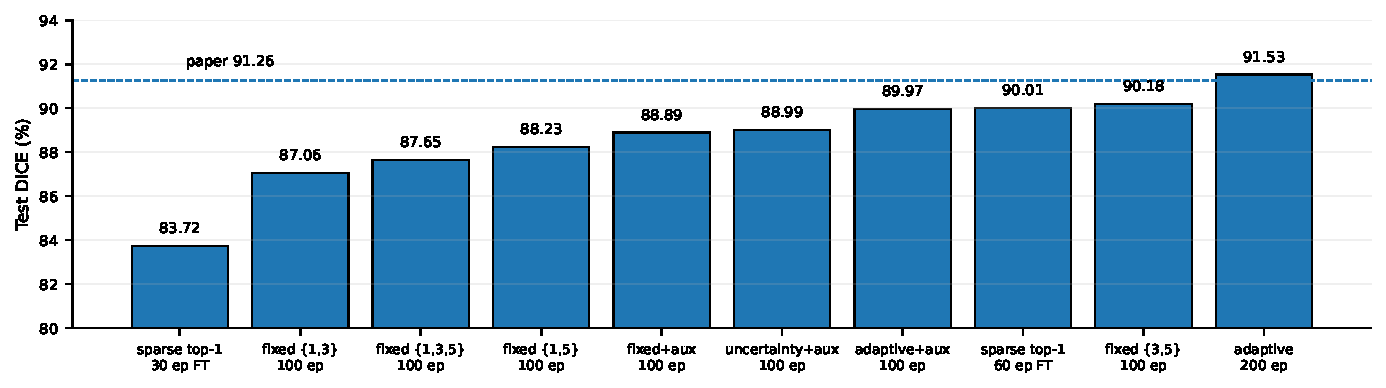
\includegraphics[width=0.94\linewidth]{figures/proposal_summary.pdf}
\caption{Completed ClinicDB runs in the preliminary study. Training budgets are shown under each bar. The dashed line is the published MK-UNet-T ClinicDB DICE of 91.26. Runs with different training budgets are not treated as directly comparable.}
\label{fig:summary}
\end{figure}

\paragraph{Interpretation} The early evidence narrows the proposal rather than proving the final method. Soft adaptive routing is worth testing further because it produced a small gain over the matched supervised control in one run. Predictive entropy did not improve routing and should remain a secondary or negative-result analysis unless multi-seed experiments change that conclusion. Sparse top-1 is more directly linked to the main efficiency question because branches are truly skipped, while routing-guided pruning offers a second route that removes router overhead completely.

\subsection{Current Limitations and Research Plan}

The current evidence has five main limitations: all extension results use one seed; most method comparisons use 100 epochs and were not fully converged; extension experiments currently use ClinicDB and MK-UNet-T only; latency was measured on a desktop CPU rather than edge hardware; and the checked repository version limits direct reproduction to the polyp pipeline. These limits are built into the next-stage plan rather than hidden.

\begin{center}\small
\renewcommand{\arraystretch}{1.08}
\begin{tabularx}{\linewidth}{@{}p{4.15cm}X@{}}
\toprule
Risk & Planned test or interpretation \\
\midrule
Small gains are seed noise & Repeat each final arm with five seeds and report variation rather than relying on one run. \\
Router selects one kernel most of the time & Use selection histograms to detect collapse; if stable, treat it as evidence for branch redundancy and test static pruning. \\
Annealing result does not generalise & Compare matched annealing schedules with equal fine-tuning budgets across both datasets. \\
Pruning result reflects faster convergence & Repeat pruned and full models to a converged budget before making an accuracy claim. \\
Sparse latency gain does not transfer & Measure target edge hardware and report CPU-only gains as CPU-only if they do not transfer. \\
Entropy conditioning remains unhelpful & Report the negative result and keep the main method focused on sparse execution and pruning. \\
\bottomrule
\end{tabularx}
\end{center}

The project is planned over five months. Month 1 will refresh the novelty review, port the experiments to GPU, repeat the main arms with full training budgets and five seeds, and test paper-exact versus repository-default settings on ColonDB. Month 2 will test matched annealing schedules, sparse top-1 on both datasets, edge-device latency, and lower-cost routers. Month 3 will repeat routing-guided pruning across datasets and test combined pruned and sparse models. Month 4 will study calibration, error detection, cross-dataset transfer, and qualitative routing or failure maps. Month 5 will consolidate the ablations, add a second modality if a reliable data pipeline is available, and prepare the manuscript.

Even if the main accuracy hypotheses are not supported, the study can still answer whether explicit conditional branch execution is practical at the 0.03 M-parameter scale, how FLOP savings relate to real latency, and whether routing statistics can help produce a smaller static MK-UNet. Negative results, including the current entropy-routing result, will be reported rather than hidden.


{\footnotesize
\renewcommand{\em}{}
\bibliographystyle{plain}
\bibliography{references}
}

\end{document}
